\documentclass[11pt,a4paper]{article}

\usepackage[margin=1in]{geometry}
\usepackage{amsmath,amssymb}
\usepackage{graphicx}
\usepackage{booktabs}
\usepackage{float}
\usepackage{caption}
\usepackage{fancyhdr}
\usepackage{setspace}
\usepackage[hidelinks]{hyperref}
\usepackage{url}

\graphicspath{{../figures/}}
\setstretch{1.15}
\captionsetup{font=small,labelfont=bf}

\pagestyle{fancy}
\fancyhf{}
\lhead{Glucose--Insulin Regulatory Kinetics}
\rhead{MAC F314 -- Team 6}
\cfoot{\thepage}

\newcommand{\Gb}{G_b}
\newcommand{\Ib}{I_b}
\newcommand{\cs}{c^{*}}

% github link
\newcommand{\repourl}{https://github.com/akshith27hiremath/Group6MathematicalModelling}

\begin{document}

%======================================================================
\begin{titlepage}
\centering
\vspace*{1cm}
{\Large Mathematical Modelling (MAC F314)\par}
\vspace{0.4cm}
{\large Group Project Report\par}
\vspace{1.8cm}
\rule{\linewidth}{1pt}\par\vspace{0.4cm}
{\LARGE\bfseries Glucose--Insulin Regulatory Kinetics\par}
\vspace{0.3cm}
{\large Modelling blood sugar control after a meal using coupled ODEs\par}
\vspace{0.3cm}
\rule{\linewidth}{1pt}\par
\vspace{1.5cm}
{\large\bfseries Project Topic 6 \quad -- \quad Team 6\par}
\vspace{1.2cm}
\begin{tabular}{lll}
\toprule
\textbf{Name} & \textbf{ID Number} & \textbf{Role} \\
\midrule
Akshith Hiremath & 2024ADPS2001H & Endocrine Modeler \\
Snigdha Kanduri & 2024ADPS2023H & Linearization Specialist \\
Nairit Bansal & 2024ADPS0037H & Eigenvalue Analyst \\
Jayaditya Kushwah & 2024ADPS0188H & Simulation Coder \\
Aluri Venkata Sai Anirudh & 2023B2AD0824H & Simulation Coder \\
Khushal Kadyan & 2024ADPS0181H & Trajectory Visualizer \\
Shaan Sharma & 2023B1AD0949H & Biological Interpreter \\
\bottomrule
\end{tabular}
\vfill
{\large Submitted to: Prof.\ Santanu Koley\par}
\vspace{0.3cm}
{\large Department of Mathematics, BITS Pilani, Hyderabad Campus\par}
\vspace{0.3cm}
{\large 20 November 2026\par}
\end{titlepage}

%======================================================================
\begin{abstract}
\noindent
After a meal, blood glucose goes up sharply, but in a healthy person it comes back to around $90$\,mg/dL within an hour or two. This happens because of a feedback loop between glucose and insulin. In this project we model that loop with two coupled ODEs, one for glucose $G(t)$ and one for insulin $I(t)$, and treat the meal as an impulse added to the glucose equation. We find the fasting equilibrium, linearise the system around it and get the characteristic equation $\lambda^2+(\alpha+d)\lambda+(\alpha d+\beta c)=0$. The equilibrium turns out to be stable for any insulin production rate $c$. What $c$ changes is the way glucose comes back. Below the critical value $\cs=(\alpha-d)^2/4\beta\approx0.0119$ the eigenvalues are real and glucose decays straight back (a stable node). Above it the eigenvalues are complex and glucose overshoots and oscillates a little before settling (a stable spiral). We solved the model with our own RK4 code and checked it against SciPy. The simulations and phase-plane plots agree with the eigenvalue analysis. Finally we set the insulin production to zero to model Type-1 diabetes. In that case glucose no longer returns to $90$\,mg/dL and instead rises to a new equilibrium at $360$\,mg/dL.
\end{abstract}

\tableofcontents
\newpage

%======================================================================
\section{Introduction}

Glucose is the main energy source for the brain and most of the body, and its level in the blood has to stay within fairly tight limits. Fasting glucose in a healthy adult is about $70$--$100$\,mg/dL, and even after a big meal it does not usually go much above $140$\,mg/dL. Very low glucose (hypoglycaemia, below about $70$\,mg/dL) causes dizziness and confusion, and in bad cases fits or loss of consciousness. Glucose that stays high for a long time (hyperglycaemia) slowly damages the blood vessels, kidneys, nerves and eyes, which is what happens in uncontrolled diabetes.

The body keeps glucose in this range using negative feedback. When glucose rises, the pancreas releases insulin. Insulin makes the muscles and fat cells take up glucose, so glucose falls, and as glucose falls the pancreas releases less insulin. Two quantities affecting each other continuously in time is exactly the kind of situation a system of two coupled ODEs is meant for, which is why we chose this approach.

The problem statement asks us to:
\begin{enumerate}
\item build a two-variable coupled ODE model for blood glucose and insulin;
\item linearise it and use the characteristic equation to decide whether the equilibrium is a node or a spiral;
\item solve the ODEs numerically with a step-based method, with an impulse function for a meal;
\item see how the behaviour depends on the insulin production rate, and find when the return to normal is a direct decay (real eigenvalues) and when it is a damped oscillation (complex eigenvalues);
\item plot the time series and phase-plane trajectories;
\item (optional) model Type-1 diabetes by setting insulin production to zero.
\end{enumerate}

The course topics we use are modelling with systems of ODEs, existence and uniqueness of solutions, linearisation and eigenvalues, classification of equilibria in the plane and phase-plane analysis (Modules 1 and 5).

%======================================================================
\section{Biological Background}

The main processes in the glucose--insulin loop are:
\begin{itemize}
\item \textbf{Glucose input.} Glucose comes into the blood from the gut after a meal. The liver also releases glucose all the time, so that the brain keeps getting fuel between meals.
\item \textbf{Uptake that does not need insulin.} The brain and red blood cells take up glucose whether or not insulin is present. This rate is roughly proportional to $G$.
\item \textbf{Uptake that needs insulin.} Muscle and fat cells only take up glucose properly when insulin is present. The more glucose and the more insulin there are, the faster this happens, so the simplest model is a term proportional to $G\cdot I$.
\item \textbf{Insulin secretion.} The $\beta$-cells of the pancreas release a small basal amount of insulin all the time, and much more when glucose goes above its normal level.
\item \textbf{Insulin clearance.} The liver and kidneys remove insulin quickly. Its half-life in the blood is only about $5$--$10$ minutes.
\end{itemize}
So high glucose leads to more insulin, which brings glucose down, which then reduces insulin again. Insulin takes some time to build up and to be cleared, so the correction can come slightly late and push glucose a bit below normal. This delay is where the oscillations we study later come from.

In Type-1 diabetes the immune system destroys the $\beta$-cells, so the body makes almost no insulin. In Type-2 diabetes the cells respond poorly to insulin and the pancreas gradually cannot keep up.

People have been modelling this system for a long time. Bolie \cite{bolie} used a linear two-equation model and Ackerman et al.\ \cite{ackerman} used a similar model to explain the shape of glucose tolerance test curves. Our model is close to Bolie's, but with the nonlinear $G\cdot I$ uptake term.

%======================================================================
\section{Mathematical Model}\label{sec:model}

\subsection{Assumptions}
We assume that:
\begin{enumerate}
\item glucose and insulin are well mixed in the blood, so each can be described by a single concentration depending only on time;
\item the liver releases glucose at a constant rate $R_0$;
\item insulin-independent uptake is $bG$ and insulin-dependent uptake is $aGI$;
\item insulin secretion is a basal amount $s_0$ plus $c\,(G-\Gb)$, where $c$ is the insulin production rate, and secretion can never be negative;
\item insulin is cleared at the rate $dI$;
\item a meal adds a total of $D$ mg/dL of glucose over a short time.
\end{enumerate}

\subsection{Variables and parameters}

\begin{table}[H]
\centering
\caption{Variables and parameters (time in minutes).}
\label{tab:params}
\small
\begin{tabular}{llll}
\toprule
Symbol & Meaning & Value & Units \\
\midrule
$G(t)$ & blood glucose & -- & mg/dL \\
$I(t)$ & plasma insulin & -- & $\mu$U/mL \\
$\Gb$ & fasting glucose & $90$ & mg/dL \\
$\Ib$ & fasting insulin & $10$ & $\mu$U/mL \\
$b$ & insulin-independent uptake rate & $0.005$ & min$^{-1}$ \\
$a$ & insulin-dependent uptake rate & $0.0015$ & mL\,$\mu$U$^{-1}$\,min$^{-1}$ \\
$c$ & insulin production rate (varied) & $0.04$ (normal) & ($\mu$U/mL)(mg/dL)$^{-1}$min$^{-1}$ \\
$d$ & insulin clearance rate & $0.1$ & min$^{-1}$ \\
$R_0$ & glucose release by the liver & $1.8$ & mg\,dL$^{-1}$\,min$^{-1}$ \\
$s_0$ & basal insulin secretion & $1.0$ & $\mu$U\,mL$^{-1}$\,min$^{-1}$ \\
$D$ & glucose added by the meal & $60$ & mg/dL \\
$t_m$ & time of the meal & $20$ & min \\
$\tau$ & length of the meal pulse & $5$ & min \\
\bottomrule
\end{tabular}
\end{table}

We picked these values so that the results are in a realistic range. For example $d=0.1$ gives an insulin half-life of $\ln2/0.1\approx6.9$ minutes, which is within the measured $5$--$10$ minutes, and a rise of about $60$\,mg/dL is typical after a normal meal.

\subsection{The equations}
Putting the assumptions together gives
\begin{align}
\frac{dG}{dt} &= R_0 - bG - aGI + M(t), \label{eq:G}\\[4pt]
\frac{dI}{dt} &= \max\{0,\; s_0 + c\,(G-\Gb)\} - dI, \label{eq:I}
\end{align}
with $G(0)=\Gb$ and $I(0)=\Ib$. The first equation says glucose goes up because of the liver and the meal and goes down because of the two kinds of uptake. The second says insulin is produced in response to glucose and is cleared at a constant rate. The two equations are coupled both ways: $I$ appears in the glucose equation through $-aGI$, and $G$ appears in the insulin equation through the secretion term. This two-way coupling is the feedback loop.

The $\max\{0,\cdot\}$ is there because if glucose falls a lot, the formula $s_0+c(G-\Gb)$ would become negative, and the pancreas obviously cannot remove insulin. This only happens when $G<\Gb-s_0/c$, which is far from the equilibrium for normal values of $c$. So it has no effect on the linear analysis below, but it does matter for some of the large-$c$ simulations.

\subsection{Meal impulse}
Ideally a meal would be a delta function,
\begin{equation}
M(t) = D\,\delta(t-t_m),
\end{equation}
which makes $G$ jump by $D$ at $t=t_m$. A numerical solver cannot handle a delta function directly, so we use a rectangular pulse with the same area:
\begin{equation}\label{eq:pulse}
M(t) = \begin{cases} D/\tau, & t_m \le t < t_m+\tau,\\ 0, & \text{otherwise,} \end{cases}
\qquad\text{so that}\qquad \int M(t)\,dt = D .
\end{equation}
As $\tau\to0$ this approaches the delta function. We used $\tau=5$ minutes, which is short compared to the time scales of the system.

\subsection{Choosing $R_0$ and $s_0$}
We want $(\Gb,\Ib)$ to be the equilibrium when there is no meal. Putting $G=\Gb$, $I=\Ib$ and $M=0$ into \eqref{eq:G}--\eqref{eq:I} and setting both derivatives to zero gives
\begin{align}
R_0 &= b\Gb + a\Gb\Ib = 0.45 + 1.35 = 1.8, \\
s_0 &= d\Ib = 1.0 .
\end{align}
With these values the equilibrium is at $(90,10)$ no matter what $c$ is. This is useful because when we change $c$ later, only the way the system returns to equilibrium changes, not where it returns to.

\subsection{Nullclines and the equilibrium}
With $M=0$, the nullclines are
\begin{align}
\frac{dG}{dt}=0:&\qquad I = \frac{R_0 - bG}{aG}, \label{eq:Gnull}\\
\frac{dI}{dt}=0:&\qquad I = \frac{1}{d}\max\{0,\; s_0 + c(G-\Gb)\}. \label{eq:Inull}
\end{align}
The first one is decreasing in $G$ and the second one is increasing (or flat), so they can only cross once. Hence $(\Gb,\Ib)$ is the only equilibrium for $c>0$.

Between the start and end of the meal $M(t)$ is constant and the right-hand side is made of polynomials and a $\max$ function, which are locally Lipschitz. So by the Picard--Lindel\"of theorem \cite{boyce} a unique solution exists locally on each piece, and we join the pieces at the meal times.


%======================================================================
\section{Linearisation and Eigenvalue Analysis}\label{sec:linear}

\subsection{Jacobian}
Let $x=G-\Gb$ and $y=I-\Ib$ be the deviations from the fasting values. Near the equilibrium the max function is not active, so we can write $f(G,I)=R_0-bG-aGI$ and $g(G,I)=s_0+c(G-\Gb)-dI$. The partial derivatives are
\[
\frac{\partial f}{\partial G}=-b-aI,\qquad
\frac{\partial f}{\partial I}=-aG,\qquad
\frac{\partial g}{\partial G}=c,\qquad
\frac{\partial g}{\partial I}=-d .
\]
At $(\Gb,\Ib)$ we define
\begin{equation}\label{eq:alphabeta}
\alpha = b + a\Ib, \qquad \beta = a\Gb,
\end{equation}
so the Jacobian is
\begin{equation}\label{eq:J}
J=\begin{pmatrix} -\alpha & -\beta \\ c & -d \end{pmatrix}
\end{equation}
and the linearised system (with the meal) is
\begin{equation}\label{eq:linear}
\frac{dx}{dt} = -\alpha x - \beta y + M(t),\qquad \frac{dy}{dt} = c\,x - d\,y .
\end{equation}
For our values, $\alpha=0.005+0.0015\times10=0.02$, $\beta=0.0015\times90=0.135$ and $d=0.1$.

$\alpha$ is the total rate at which glucose is removed at the fasting state, and $\beta$ measures how strongly extra insulin lowers glucose. The off-diagonal entries have opposite signs ($-\beta<0$ and $c>0$): insulin lowers glucose, but glucose raises insulin. That is what negative feedback looks like in the Jacobian.

\subsection{Characteristic equation}
The eigenvalues come from $\det(J-\lambda I)=0$:
\[
\det\begin{pmatrix}-\alpha-\lambda & -\beta\\ c & -d-\lambda\end{pmatrix}
=(\alpha+\lambda)(d+\lambda)+\beta c = 0,
\]
which gives
\begin{equation}\label{eq:char}
\boxed{\;\lambda^2 + (\alpha+d)\,\lambda + (\alpha d + \beta c) = 0\;}
\end{equation}
This is $\lambda^2-(\operatorname{tr}J)\lambda+\det J=0$ with
\begin{equation}
\operatorname{tr}J = -(\alpha+d),\qquad \det J = \alpha d+\beta c,
\end{equation}
and the roots are
\begin{equation}\label{eq:roots}
\lambda_{1,2} = \frac{-(\alpha+d) \pm \sqrt{\Delta}}{2},\qquad \Delta=(\operatorname{tr}J)^2-4\det J .
\end{equation}

\subsection{Stability}
All the parameters are positive, so $\operatorname{tr}J<0$ and $\det J>0$ for every $c\ge0$. This means both eigenvalues have negative real parts and the equilibrium is asymptotically stable. Since neither eigenvalue has zero real part, the Hartman--Grobman theorem \cite{boyce} tells us that the nonlinear system behaves the same way near the equilibrium.

So glucose always comes back to normal in this model. The interesting question is how it comes back. Notice also that the trace does not depend on $c$ at all. Only the determinant does.

\subsection{The critical value $\cs$}
Expanding the discriminant,
\begin{align}
\Delta &= (\alpha+d)^2 - 4(\alpha d+\beta c) \nonumber\\
       &= (\alpha-d)^2 - 4\beta c. \label{eq:disc}
\end{align}
This decreases as $c$ increases and becomes zero at
\begin{equation}\label{eq:cstar}
\boxed{\;\cs = \frac{(\alpha-d)^2}{4\beta}\;}
\end{equation}
So we get three cases:
\begin{itemize}
\item $c<\cs$: $\Delta>0$, two real negative eigenvalues, \textbf{stable node}. Glucose decays back without oscillating.
\item $c=\cs$: $\Delta=0$, one repeated eigenvalue $-(\alpha+d)/2$, \textbf{degenerate node} (critical damping).
\item $c>\cs$: $\Delta<0$, complex eigenvalues $\lambda=\sigma\pm i\omega$ with
\begin{equation}
\sigma = -\frac{\alpha+d}{2},\qquad \omega=\frac{\sqrt{4\beta c-(\alpha-d)^2}}{2},
\end{equation}
\textbf{stable spiral}. Glucose oscillates while decaying.
\end{itemize}
With our numbers,
\[
\cs = \frac{(0.02-0.1)^2}{4\times0.135} = \frac{0.0064}{0.54} \approx 0.01185 .
\]
Our normal value $c=0.04$ is about $3.4$ times this, so the healthy case in our model is a spiral.

It also helps to compare \eqref{eq:char} with the damped oscillator equation $\lambda^2+2\zeta\omega_n\lambda+\omega_n^2=0$. This gives
\begin{equation}\label{eq:zeta}
\omega_n=\sqrt{\alpha d+\beta c},\qquad
\zeta=\frac{\alpha+d}{2\sqrt{\alpha d+\beta c}} ,
\end{equation}
where $\zeta$ is the damping ratio. $\zeta>1$ when $c<\cs$ (overdamped), $\zeta=1$ at $c=\cs$, and $\zeta<1$ when $c>\cs$ (underdamped). As $c$ gets very large, $\zeta\to0$, so the response gets more and more oscillatory but never becomes unstable.

\subsection{Eigenvalues for our parameter values}
Table~\ref{tab:eig} gives the eigenvalues for the five values of $c$ we simulated. We calculated them from \eqref{eq:roots} and also with \texttt{numpy.linalg.eigvals}, and both gave the same answers.

\begin{table}[H]
\centering
\caption{Eigenvalues for different insulin production rates ($\alpha=0.02$, $\beta=0.135$, $d=0.1$, $\operatorname{tr}J=-0.12$).}
\label{tab:eig}
\begin{tabular}{cccccl}
\toprule
$c$ & $\det J$ & $\Delta$ & $\lambda_{1,2}$ (min$^{-1}$) & $\zeta$ & Type \\
\midrule
$0.004$ & $0.00254$ & $+0.00424$ & $-0.0274,\;-0.0926$ & $1.19$ & stable node \\
$\cs=0.01185$ & $0.00360$ & $0$ & $-0.0600$ (repeated) & $1.00$ & degenerate node \\
$0.04$ & $0.00740$ & $-0.0152$ & $-0.060\pm0.0616\,i$ & $0.70$ & stable spiral \\
$0.15$ & $0.02225$ & $-0.0746$ & $-0.060\pm0.1366\,i$ & $0.40$ & stable spiral \\
$0.4$ & $0.05600$ & $-0.2096$ & $-0.060\pm0.2289\,i$ & $0.25$ & stable spiral \\
\bottomrule
\end{tabular}
\end{table}

For $c=0.04$, the period of oscillation is $2\pi/\omega\approx102$ minutes and the decay time constant is $1/|\sigma|\approx16.7$ minutes. Since the decay is fast compared to the period, the oscillation dies out almost immediately. Each half-period the amplitude is multiplied by $e^{\sigma\pi/\omega}\approx0.047$. So in practice we should see one small dip below $90$ and nothing after that, which is what the simulations show.

\subsection{Exact solution of the linear system}
For a delta-function meal, let $s=t-t_m$. The meal makes $x(0)=D$ and $y(0)=0$, and after that the system has no input. Differentiating the first equation of \eqref{eq:linear} and substituting the second one (using $\beta y=-\dot x-\alpha x$) gives a single second-order equation:
\begin{equation}\label{eq:second}
\ddot x+(\alpha+d)\dot x+(\alpha d+\beta c)x=0,\qquad x(0)=D,\quad \dot x(0)=-\alpha D .
\end{equation}
This is the damped harmonic oscillator equation, and its characteristic equation is \eqref{eq:char}. Solving it in the three cases gives:

\noindent\textbf{Node} ($\Delta>0$, real roots $\lambda_1>\lambda_2$):
\begin{equation}\label{eq:sol_node}
x(s)=\frac{D}{\lambda_1-\lambda_2}\Bigl[-(\alpha+\lambda_2)\,e^{\lambda_1 s}+(\alpha+\lambda_1)\,e^{\lambda_2 s}\Bigr],\qquad
y(s)=\frac{cD}{\lambda_1-\lambda_2}\bigl(e^{\lambda_1 s}-e^{\lambda_2 s}\bigr).
\end{equation}
\textbf{Critical} ($\Delta=0$, $\sigma=-(\alpha+d)/2$):
\begin{equation}\label{eq:sol_crit}
x(s)=D\,e^{\sigma s}\Bigl(1+\frac{d-\alpha}{2}\,s\Bigr),\qquad
y(s)=cD\,s\,e^{\sigma s}.
\end{equation}
\textbf{Spiral} ($\Delta<0$):
\begin{equation}\label{eq:sol_spiral}
x(s)=D\,e^{\sigma s}\Bigl[\cos(\omega s)+\frac{d-\alpha}{2\omega}\sin(\omega s)\Bigr],\qquad
y(s)=\frac{cD}{\omega}\,e^{\sigma s}\sin(\omega s).
\end{equation}

In the spiral case, $x$ and $y$ keep changing sign, so both glucose and insulin go below their fasting values at some point. In the node case, $x(s)=0$ would need $e^{(\lambda_1-\lambda_2)s}=(\alpha+\lambda_1)/(\alpha+\lambda_2)$. Here $\alpha<d$, so both $\alpha+\lambda_1$ and $\alpha+\lambda_2$ are negative and their ratio is less than $1$, which only happens for $s<0$. So in the node case glucose never goes below the fasting level after a meal.

For the phase plane we also need the eigenvectors. From the first row of $J-\lambda I$,
\begin{equation}\label{eq:eigvec}
\mathbf{v}_i=\begin{pmatrix}\beta\\ -(\alpha+\lambda_i)\end{pmatrix}.
\end{equation}
For $c=0.004$ the slow eigenvector ($\lambda_1=-0.0274$) has slope $0.055$ and the fast one ($\lambda_2=-0.0926$) has slope $0.54$. In the node case these are straight-line solutions. The general solution is $\mathbf{X}(s)=Ve^{\Lambda s}V^{-1}\mathbf{X}(0)$, and we use this to draw the curves in Figure~\ref{fig:phase_lin}.

%======================================================================
\section{Numerical Method}\label{sec:numerics}

\subsection{RK4}
We used the classical fourth-order Runge--Kutta method \cite{boyce}. For $\mathbf{u}'=\mathbf{f}(t,\mathbf{u})$ with step $h$:
\begin{align}
\mathbf{k}_1 &= \mathbf{f}(t_n,\mathbf{u}_n),\\
\mathbf{k}_2 &= \mathbf{f}\bigl(t_n+\tfrac h2,\;\mathbf{u}_n+\tfrac h2\mathbf{k}_1\bigr),\\
\mathbf{k}_3 &= \mathbf{f}\bigl(t_n+\tfrac h2,\;\mathbf{u}_n+\tfrac h2\mathbf{k}_2\bigr),\\
\mathbf{k}_4 &= \mathbf{f}\bigl(t_n+h,\;\mathbf{u}_n+h\mathbf{k}_3\bigr),\\
\mathbf{u}_{n+1} &= \mathbf{u}_n+\frac h6\bigl(\mathbf{k}_1+2\mathbf{k}_2+2\mathbf{k}_3+\mathbf{k}_4\bigr).
\end{align}
The global error is $O(h^4)$. We used $h=0.05$ minutes, which is small compared to the time scales of the system.

Because $M(t)$ jumps at $t_m$ and $t_m+\tau$, we solve in three parts (before, during and after the meal) with $M$ constant in each part, and use the end of one part as the start of the next. This way no RK4 step goes across a jump.

To check our solver, we solved the normal case again with SciPy's \texttt{solve\_ivp}. The largest difference in glucose between the two was about $0.14$\,mg/dL, which is tiny compared to the $55$\,mg/dL rise after the meal, so our RK4 code is working correctly.

\subsection{Code}
The code is in our GitHub repository (Section~\ref{sec:repo}) and has five Python files:
\begin{itemize}
\item \texttt{model\_and\_solver.py}: the parameters, the model and its linear version, the RK4 function, the eigenvalue formula, and \texttt{meal\_sim}, which does the three-part solve;
\item \texttt{eigen\_analysis.py}: Table~\ref{tab:eig} and Figures~\ref{fig:locus}--\ref{fig:eigvsc};
\item \texttt{simulations.py}: Figures~\ref{fig:meal}, \ref{fig:sens} and \ref{fig:nl_vs_lin}, Table~\ref{tab:metrics} and the SciPy check;
\item \texttt{phase\_plane.py}: Figures~\ref{fig:phase_lin}--\ref{fig:phase_meal};
\item \texttt{type1\_diabetes.py}: Figures~\ref{fig:t1_single} and \ref{fig:t1_phase}.
\end{itemize}
\texttt{run\_all.py} runs all of them. We used NumPy and Matplotlib, and SciPy only for the check above.

%======================================================================
\section{Results}\label{sec:results}

\subsection{Response to one meal}

\begin{figure}[H]
\centering
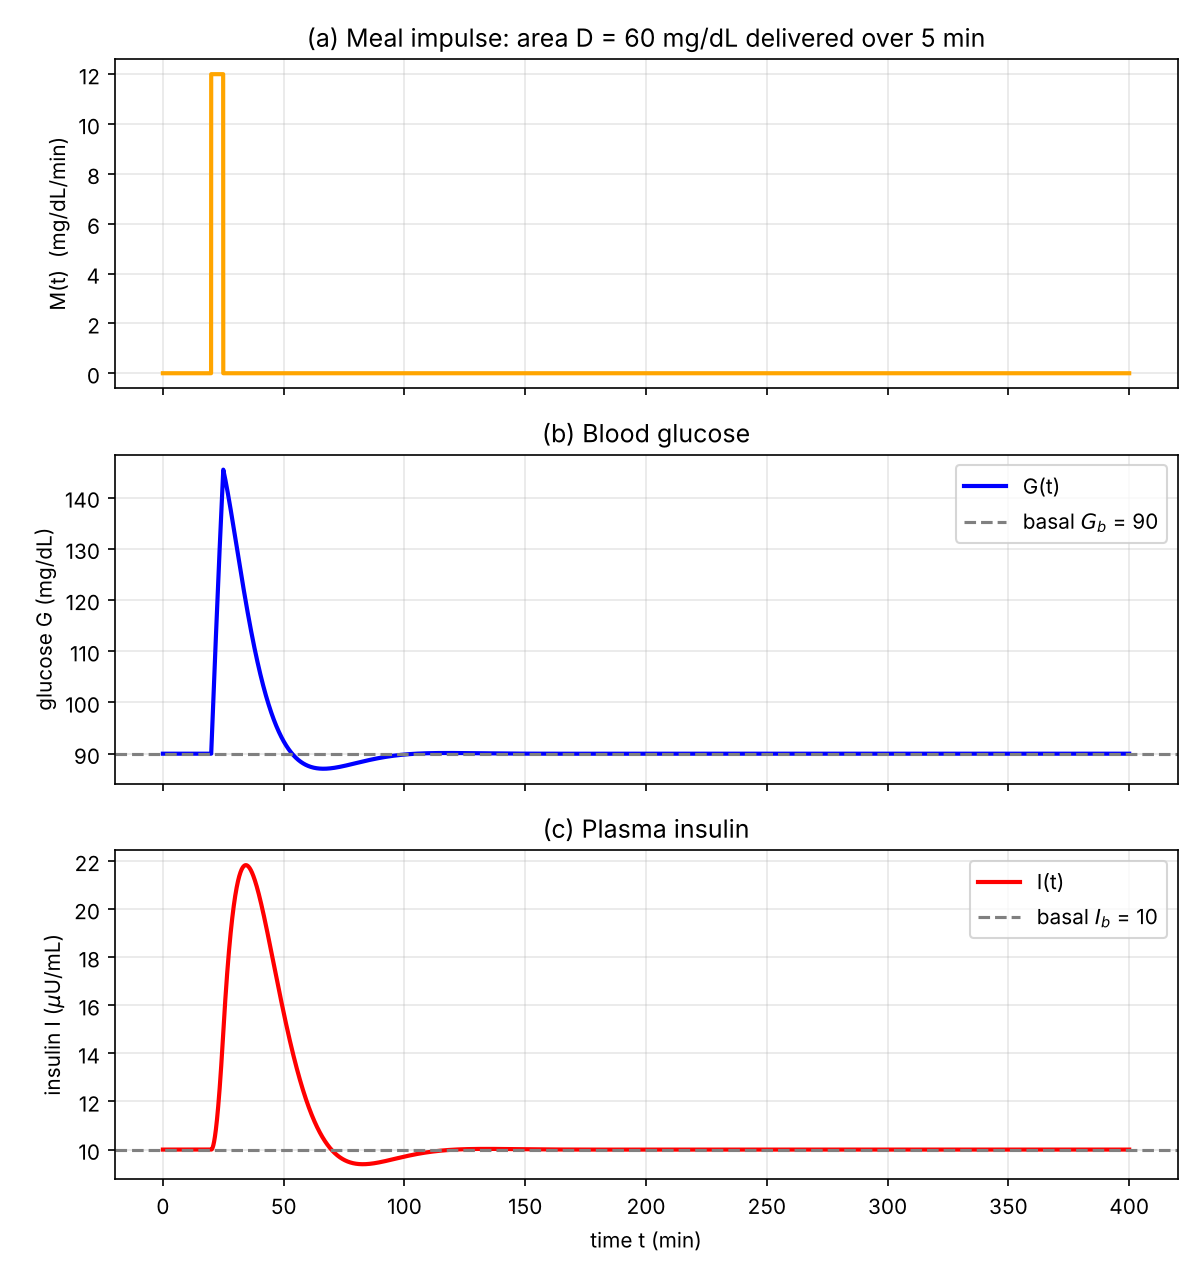
\includegraphics[width=0.82\linewidth]{fig_meal_response.png}
\caption{Response to one meal with $c=0.04$: (a) meal input, (b) glucose, (c) insulin. Dashed lines are the fasting values.}
\label{fig:meal}
\end{figure}

Figure~\ref{fig:meal} shows what happens after one meal with the normal value $c=0.04$. Before $t=20$ nothing changes, which is a good check that $(90,10)$ really is an equilibrium. During the meal glucose goes up almost linearly and reaches $145.4$\,mg/dL at $t=25$, the end of the pulse. The rise is $55.4$\,mg/dL rather than the full $60$, because insulin has already started working during those five minutes.

Glucose then falls and crosses $90$\,mg/dL at about $t=53.5$, goes slightly below to $87.1$\,mg/dL at $t=66.5$, and then settles at $90$. Two hours after the meal it is back to normal.

Insulin peaks at $21.8$\,$\mu$U/mL at $t=34.4$, about $9$ minutes after glucose peaks. This lag is because insulin has to build up through secretion and is cleared with a time constant of $1/d=10$ minutes. Since insulin is still raised when glucose gets back to $90$, glucose is pushed a little below normal. That is the small dip in panel (b). Insulin also dips slightly below $10$ before settling, as the spiral solution \eqref{eq:sol_spiral} says it should.

\subsection{Changing the insulin production rate}

\begin{figure}[H]
\centering
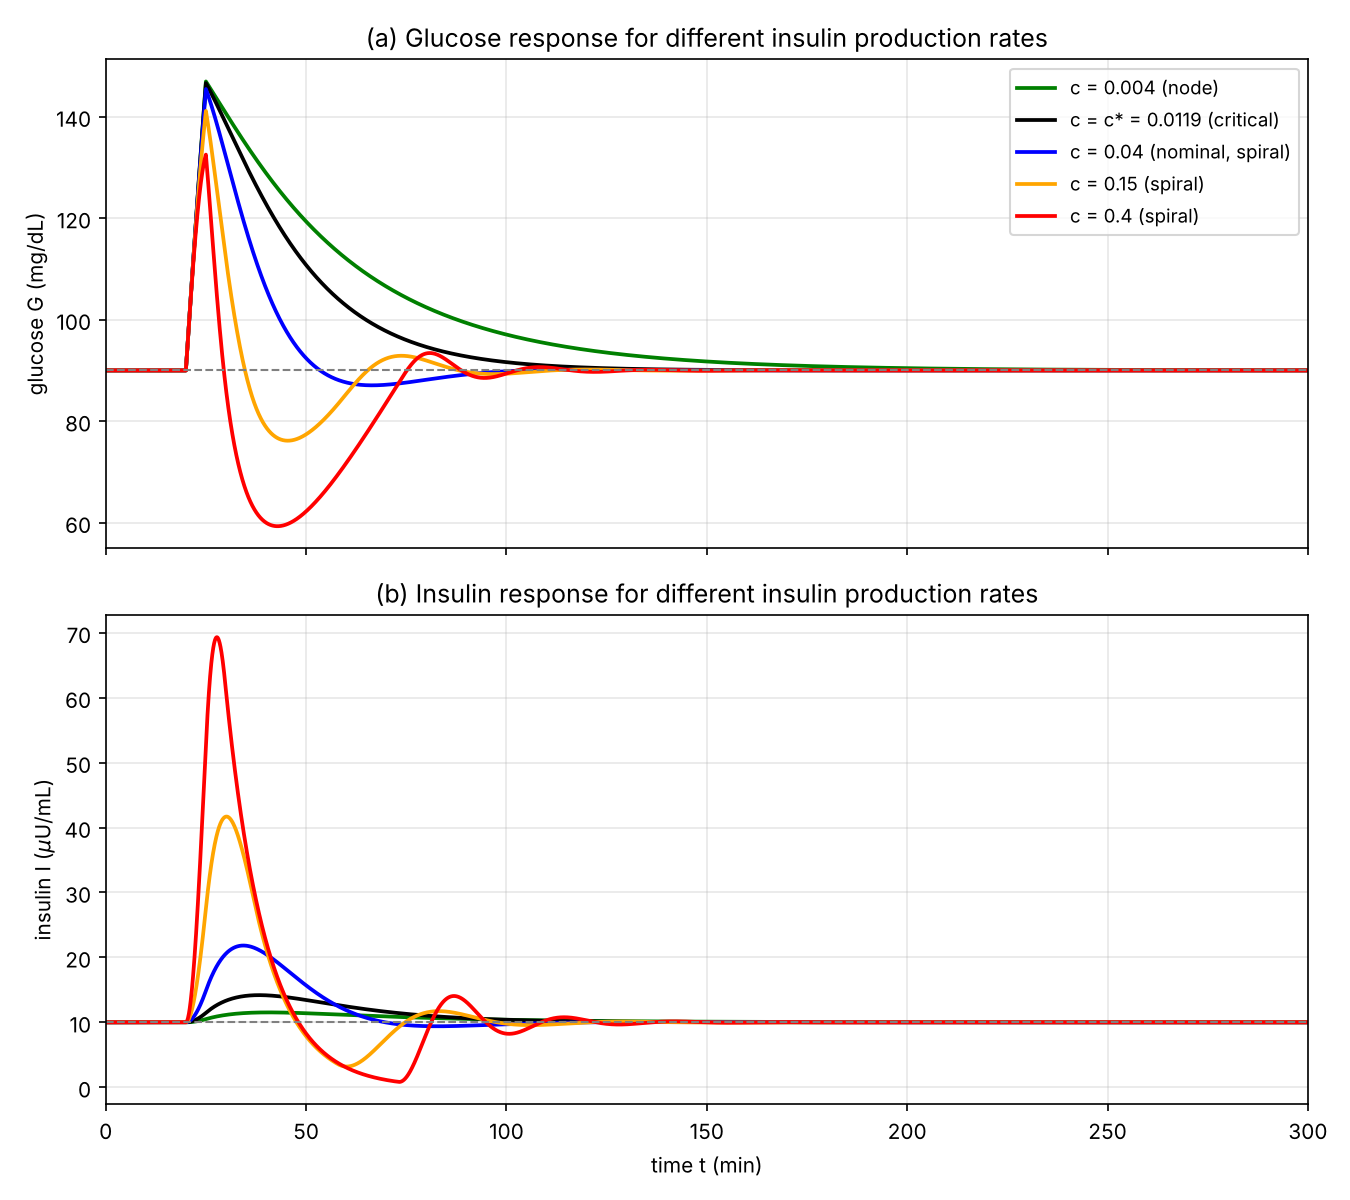
\includegraphics[width=0.85\linewidth]{fig_sensitivity_c.png}
\caption{Glucose (a) and insulin (b) after the same meal for five values of $c$: one node, the critical value and three spirals.}
\label{fig:sens}
\end{figure}

Figure~\ref{fig:sens} shows the same meal for five values of $c$. With $c=0.004$, which is below $\cs$, glucose comes down slowly and never crosses $90$. It is still about $7$\,mg/dL high at $t=100$ and $92.3$\,mg/dL two hours after the meal. This is the direct decay we expected for real eigenvalues, and it is slow because the slow eigenvalue is $-0.0274$ (time constant about $36$ minutes). At $c=\cs$ the decay is faster but there is still no dip. For $c=0.04$ there is a small dip of $2.9$\,mg/dL.

For $c=0.15$ and $c=0.4$ glucose falls quickly and overshoots a lot, down to $76$ and $59$\,mg/dL, and we can see one or two more oscillations after that. The dips also come closer together as $c$ increases, since the period gets shorter ($46$ and $27$ minutes from Table~\ref{tab:eig}). For $c=0.4$, glucose goes below $70$\,mg/dL, which counts as hypoglycaemia.

The insulin peaks increase a lot with $c$: $11.5$, $14.2$, $21.8$, $41.7$ and $69.3$\,$\mu$U/mL. For $c=0.15$ and $0.4$, insulin later drops almost to zero and the curve has a sharp corner. This is where the $\max\{0,\cdot\}$ in the secretion term switches on, i.e.\ the pancreas stops secreting completely. The linear model cannot show this. In all five cases the system ends up back at $(90,10)$.

\begin{table}[H]
\centering
\caption{Results for the five values of $c$ (meal $D=60$\,mg/dL). Settling time is measured from the start of the meal until $|G-\Gb|$ stays below $2$\,mg/dL.}
\label{tab:metrics}
\begin{tabular}{cccccc}
\toprule
$c$ & type & peak rise & undershoot & settling time & peak insulin\\
 & & (mg/dL) & (mg/dL) & (min) & ($\mu$U/mL)\\
\midrule
$0.004$ & node & $56.9$ & $0.0$ & $125.3$ & $11.5$\\
$0.0119$ & critical & $56.6$ & $0.0$ & $76.0$ & $14.2$\\
$0.04$ & spiral & $55.4$ & $2.9$ & $58.6$ & $21.8$\\
$0.15$ & spiral & $51.1$ & $13.8$ & $59.8$ & $41.7$\\
$0.4$ & spiral & $42.5$ & $30.7$ & $65.2$ & $69.3$\\
\bottomrule
\end{tabular}
\end{table}

Table~\ref{tab:metrics} puts these numbers side by side. As $c$ increases, the peak rise goes down a little and the peak insulin goes up a lot. The undershoot is zero for the node and critical cases, as the exact solution predicted, and grows quickly in the spiral region. The settling time is longest for the node and drops to about an hour for $c=0.04$, but it does not keep improving for larger $c$, because the oscillations take glucose away from $90$ again.


\subsection{Eigenvalues as $c$ changes}

\begin{figure}[H]
\centering
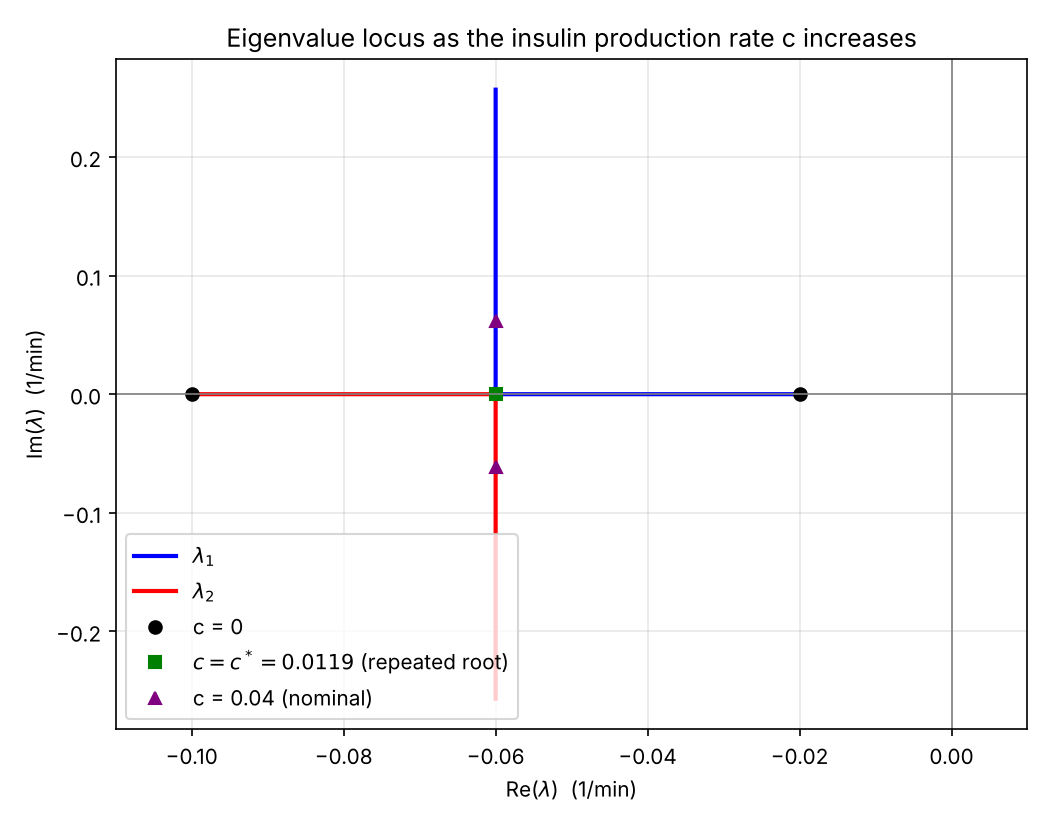
\includegraphics[width=0.7\linewidth]{fig_eigen_locus.png}
\caption{Path of the eigenvalues in the complex plane as $c$ goes from $0$ to $0.5$. Black dots are $c=0$, the green square is $c=\cs$ and the purple triangles are $c=0.04$.}
\label{fig:locus}
\end{figure}

Figure~\ref{fig:locus} shows where the eigenvalues move as $c$ increases. At $c=0$ the two equations are not coupled and the eigenvalues are $-\alpha=-0.02$ and $-d=-0.1$. As $c$ increases, they move towards each other along the real axis and meet at $-0.06$ when $c=\cs$. After that they become a complex pair and move straight up and down, because the real part stays at $-0.06$ while the imaginary part grows. They never cross into the right half-plane, so increasing insulin production can never make the system unstable.

\begin{figure}[H]
\centering
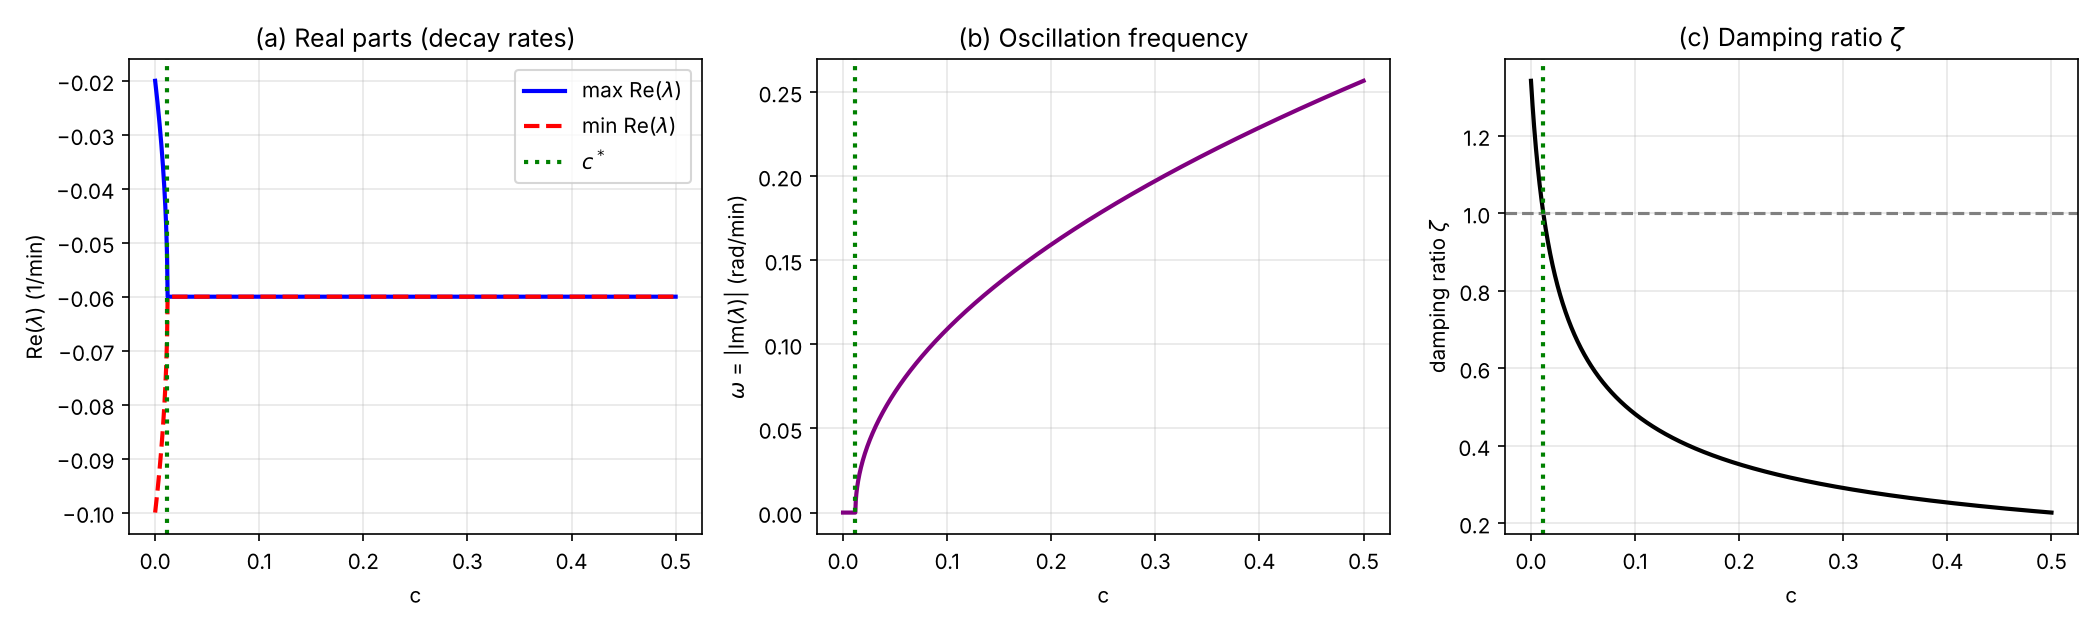
\includegraphics[width=\linewidth]{fig_eigen_vs_c.png}
\caption{(a) Real parts of the eigenvalues, (b) oscillation frequency $\omega$ and (c) damping ratio $\zeta$ against $c$. The green dotted line is $\cs$.}
\label{fig:eigvsc}
\end{figure}

Figure~\ref{fig:eigvsc} shows the same thing in terms of numbers. For $c<\cs$ the slow eigenvalue goes from $-0.02$ to $-0.06$, so increasing $c$ makes the return faster. After $\cs$ both real parts stay at $-0.06$. This means that beyond $\cs$, extra insulin production does not make the decay any faster; it only adds oscillation. This is why the settling time in Table~\ref{tab:metrics} stops improving after $c=0.04$. The frequency (b) is zero up to $\cs$ and then increases like a square root. The damping ratio (c) starts at about $1.34$, equals $1$ at $\cs$, and decreases towards $0$ after that.

\subsection{Phase plane}

\begin{figure}[H]
\centering
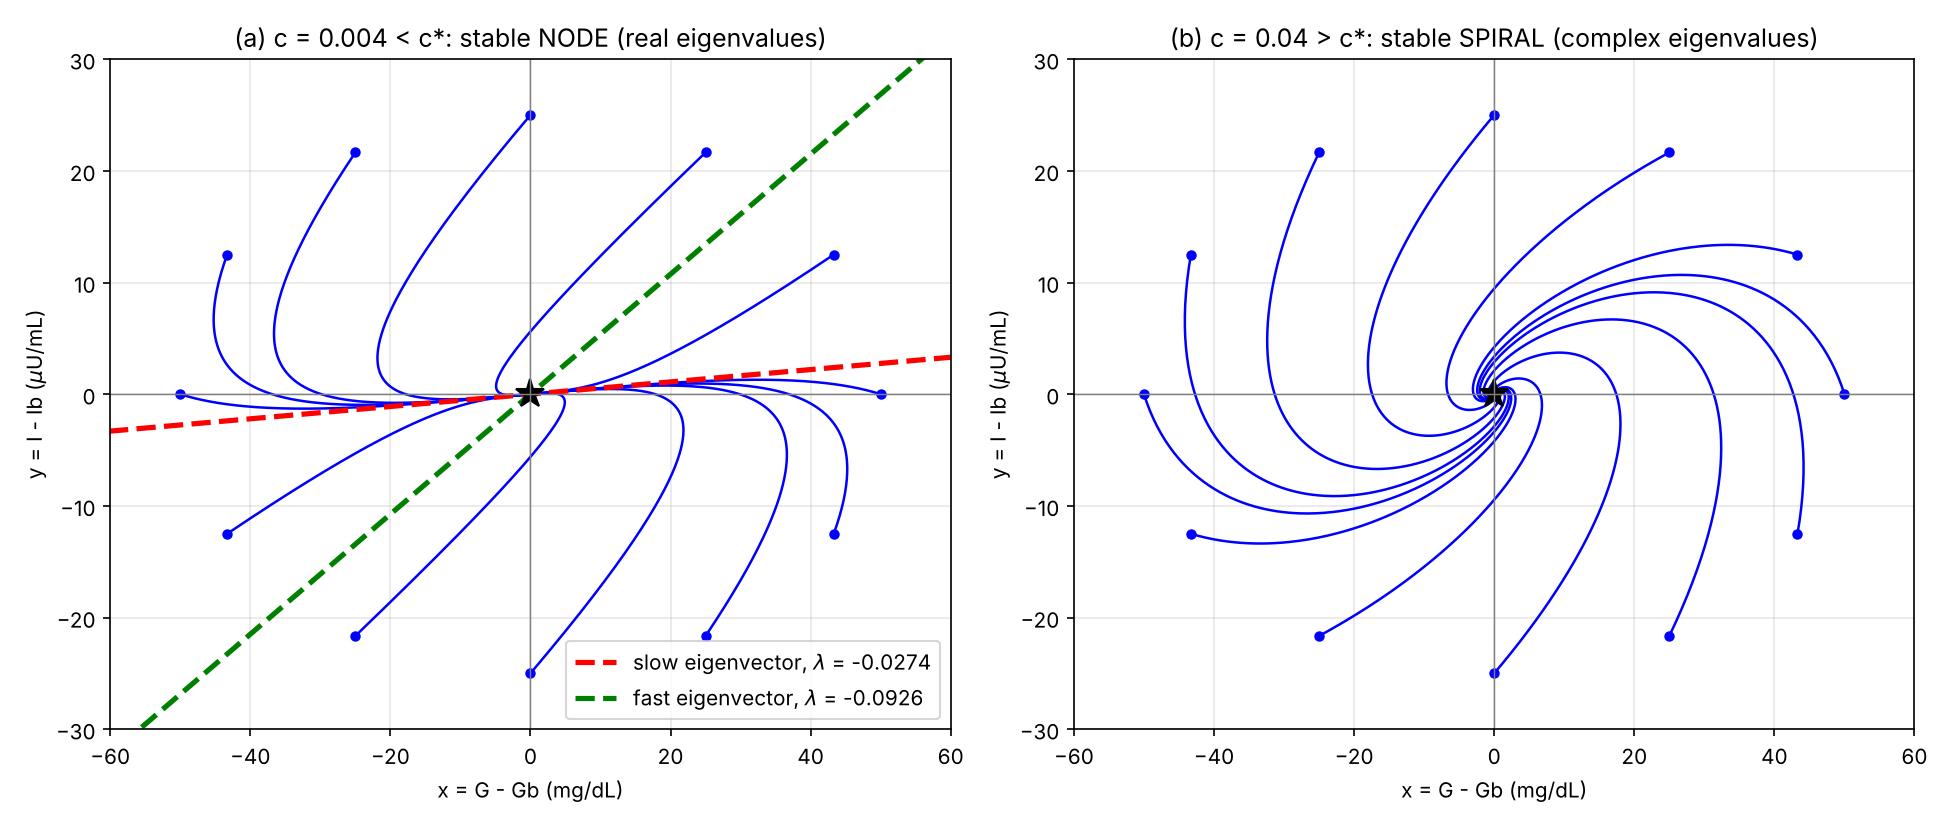
\includegraphics[width=\linewidth]{fig_phase_linear_parametric.png}
\caption{Phase curves $(x(t),y(t))$ of the linear system from $\mathbf{X}(t)=Ve^{\Lambda t}V^{-1}\mathbf{X}_0$, for twelve starting points. (a) Node, $c=0.004$, with the two eigenvector directions. (b) Spiral, $c=0.04$.}
\label{fig:phase_lin}
\end{figure}

Figure~\ref{fig:phase_lin} shows the phase curves of the linear system for a node and a spiral. In the node case (a), the dashed lines are the eigenvectors. A trajectory that starts on one of them moves straight along it into the origin. Other trajectories first move quickly in the direction of the fast eigenvector and then come into the origin along the slow eigenvector (red). This line is nearly flat, so near the end it is mostly glucose slowly coming back while insulin stays almost at its fasting value. No trajectory goes around the origin. In the spiral case (b), every trajectory curves around the origin anticlockwise as it comes in. Each time a curve crosses $x=0$, glucose is passing through $90$\,mg/dL. The spiral shrinks very fast, by a factor of about $0.002$ each full turn, so only the first half turn is visible.

\begin{figure}[H]
\centering
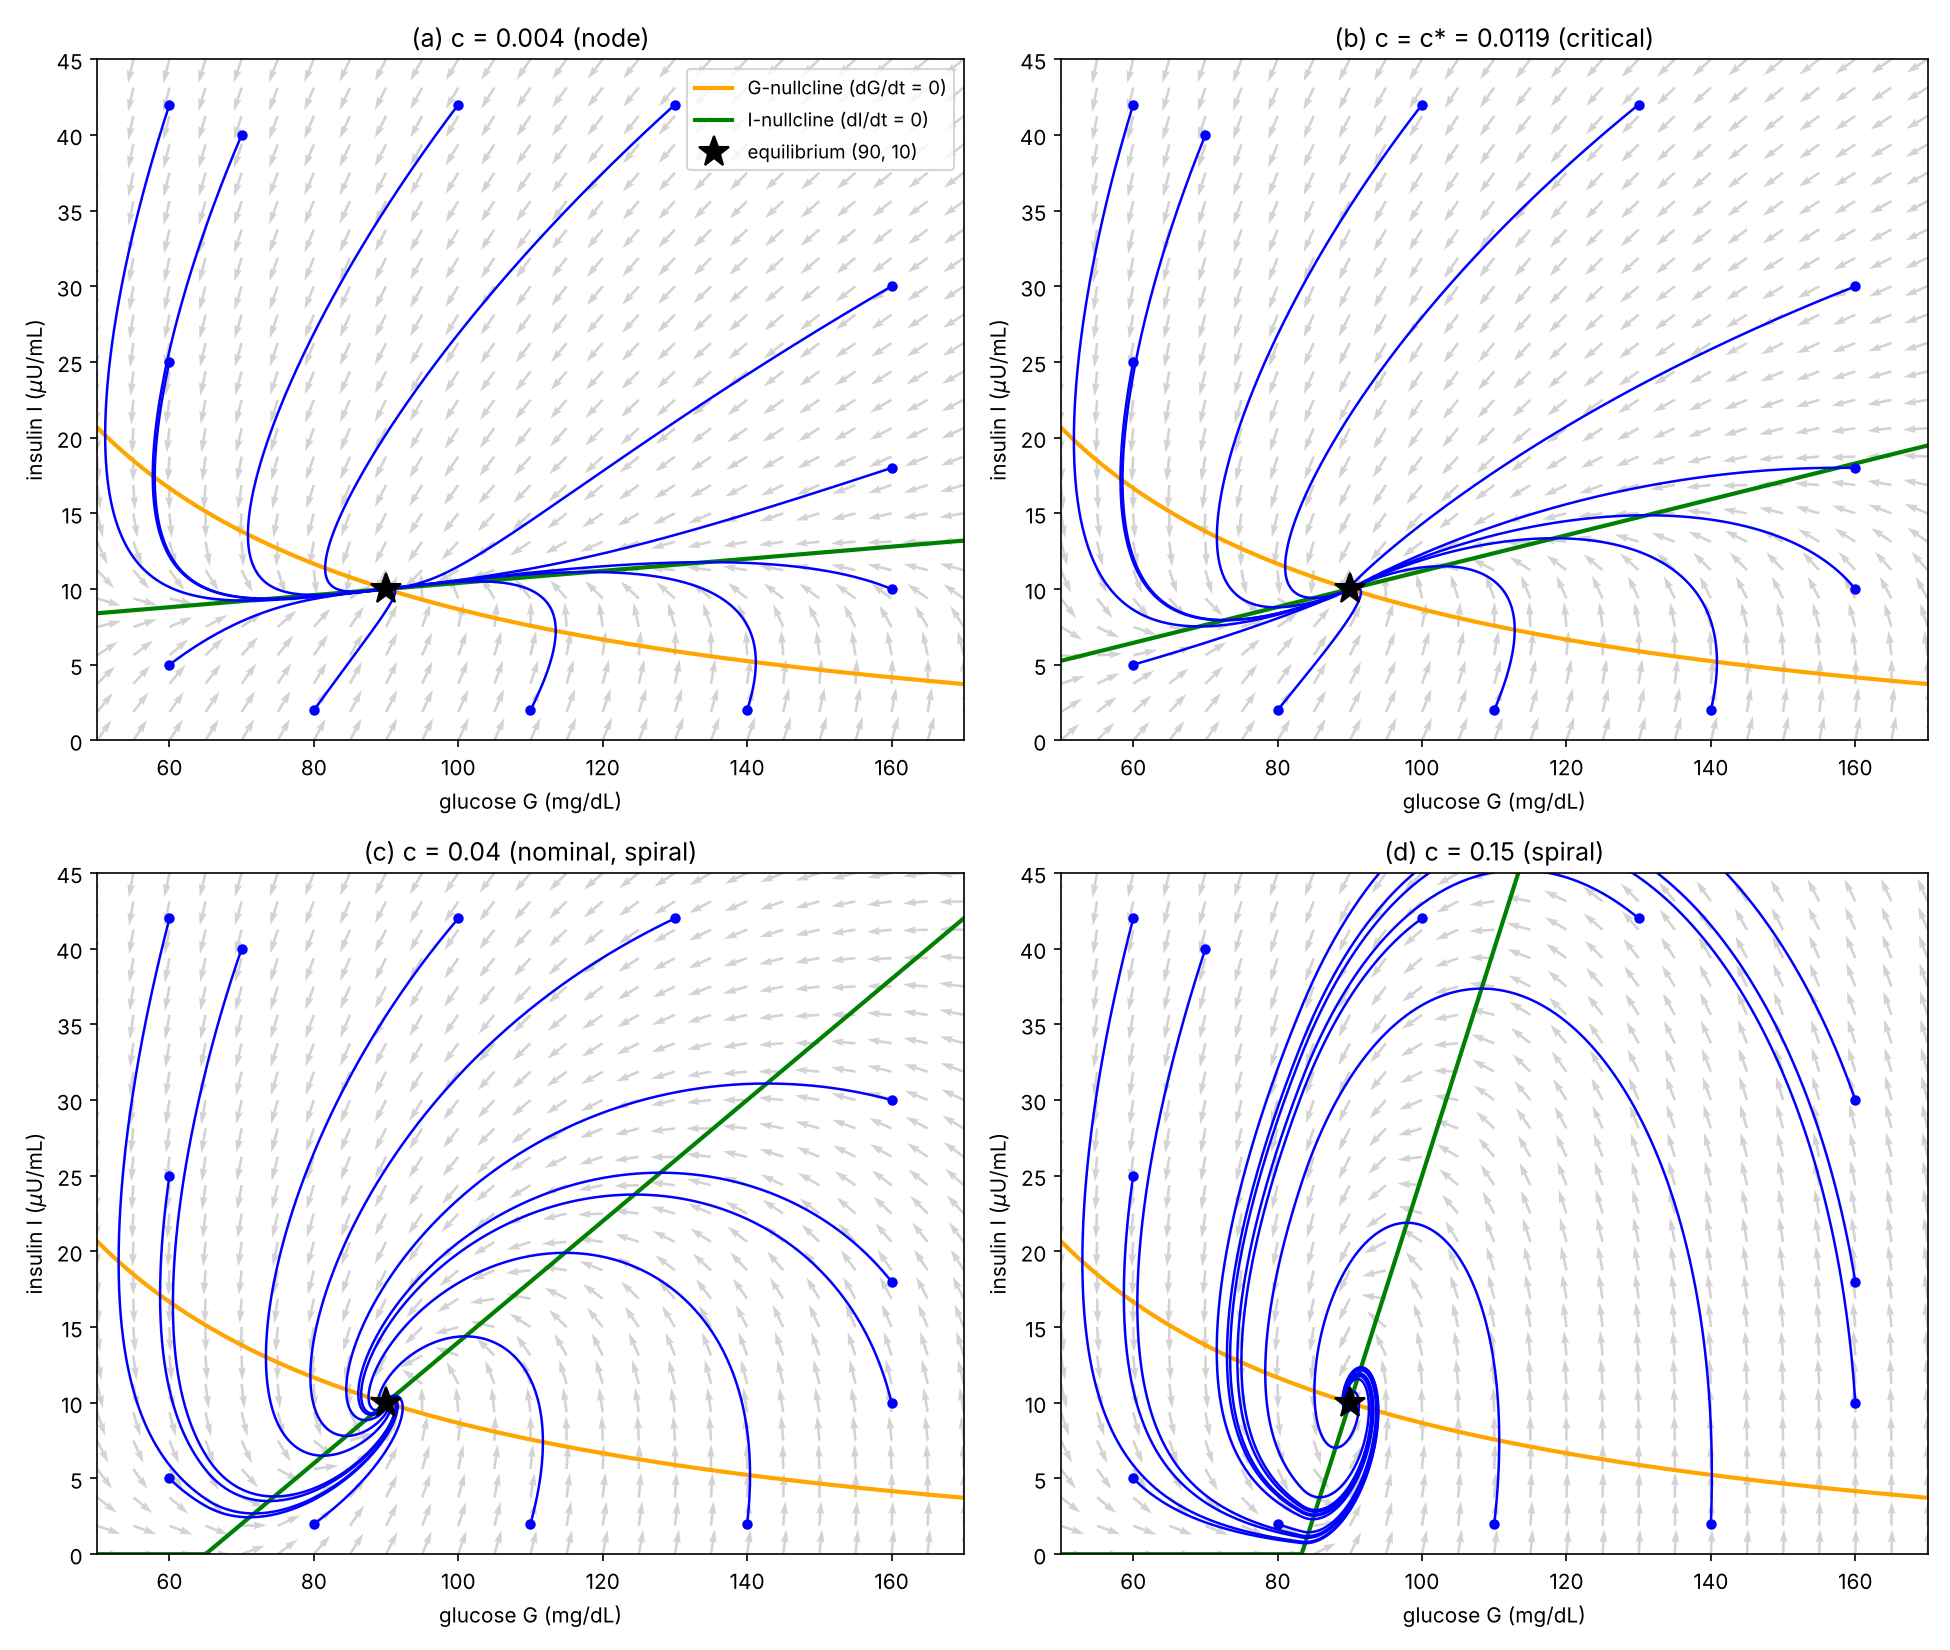
\includegraphics[width=\linewidth]{fig_phase_nonlinear.png}
\caption{Phase portraits of the nonlinear system (no meal) for (a) $c=0.004$, (b) $c=\cs$, (c) $c=0.04$ and (d) $c=0.15$. Grey arrows show the direction field, orange is the $G$-nullcline, green is the $I$-nullcline and blue curves are trajectories from twelve starting points.}
\label{fig:phase_nl}
\end{figure}

Figure~\ref{fig:phase_nl} is the same idea for the full nonlinear model, with direction fields and nullclines added. In every panel the nullclines only meet once, at $(90,10)$, as we argued in Section~\ref{sec:model}. Trajectories cross the $G$-nullcline vertically and the $I$-nullcline horizontally, as they should. In (a) and (b) the trajectories first move almost vertically (insulin adjusts quickly), then follow the $I$-nullcline slowly into the equilibrium without circling it. In (c) they curve around the equilibrium a little before entering. In (d), with $c=0.15$, the loops are much bigger: high glucose causes a large insulin spike, glucose then drops below $90$, insulin falls almost to zero, and glucose recovers. Far from the equilibrium the picture is not symmetric like the linear one, because of the $aGI$ term and the cut-off at zero secretion.

\begin{figure}[H]
\centering
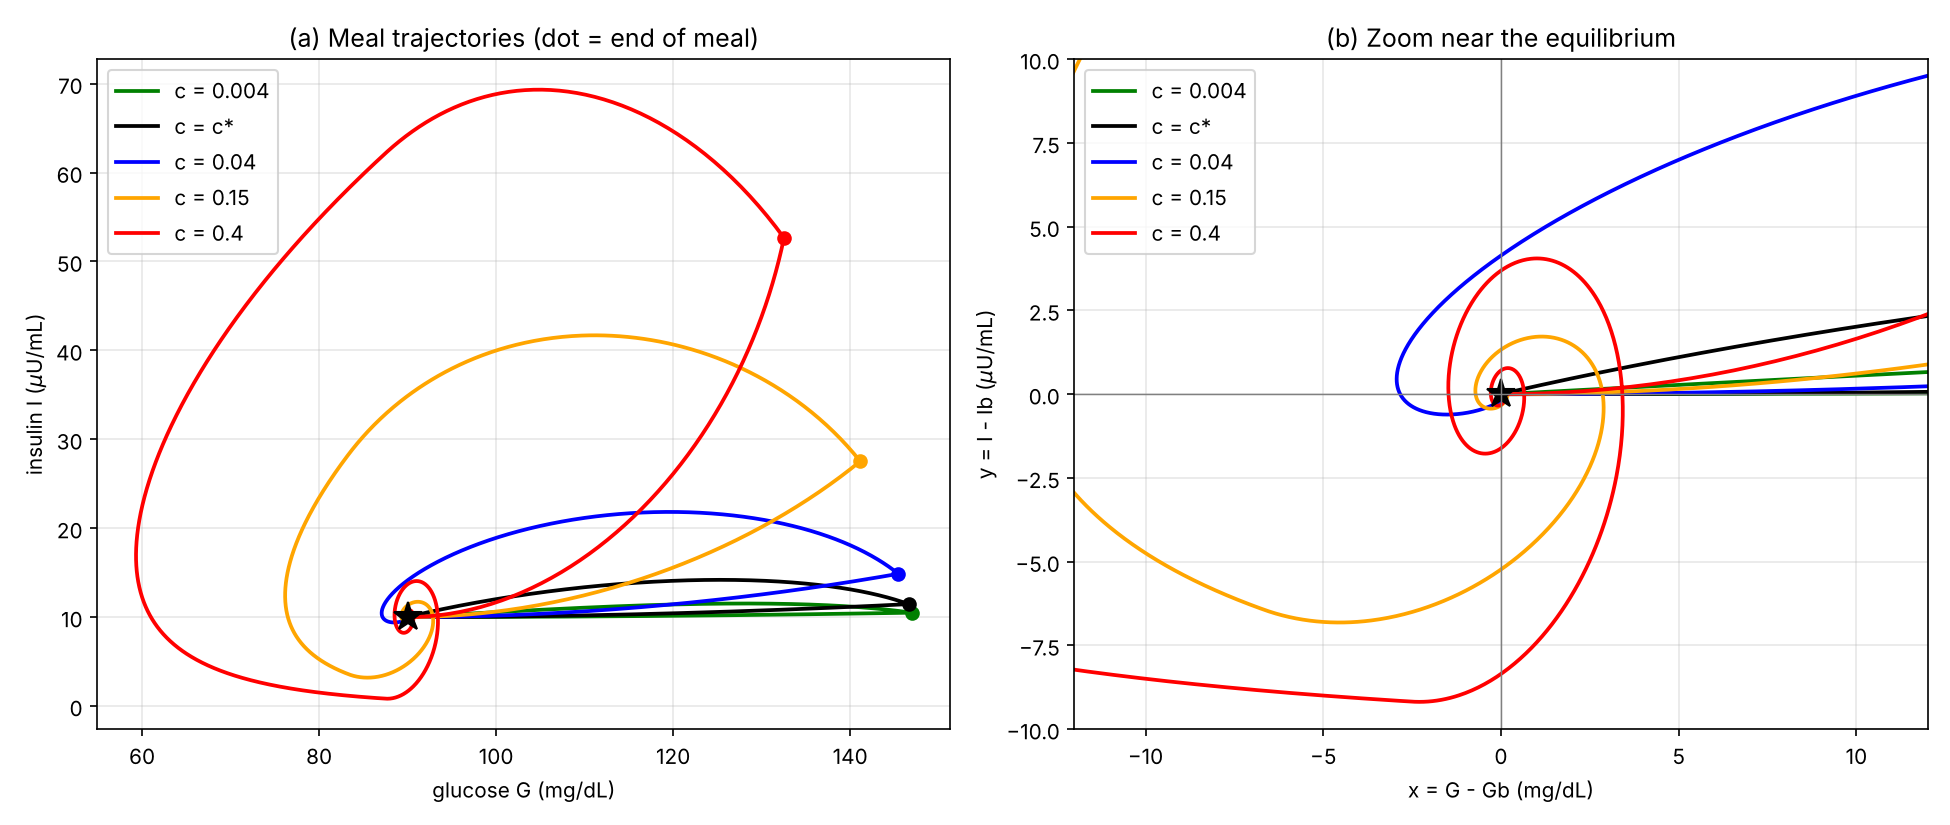
\includegraphics[width=\linewidth]{fig_phase_meal.png}
\caption{(a) The meal simulations of Figure~\ref{fig:sens} plotted in the $(G,I)$ plane; dots mark the end of the meal. (b) Close-up near the equilibrium.}
\label{fig:phase_meal}
\end{figure}

In Figure~\ref{fig:phase_meal} we plotted the actual meal simulations from Figure~\ref{fig:sens} in the phase plane. During the meal all curves move almost horizontally to the right, because glucose rises before insulin has responded. After the meal, the curves for small $c$ come back fairly directly without looping around. For larger $c$ there is a big loop: insulin rises, glucose drops below $90$, insulin falls, and the curve spirals in. The close-up in (b) shows the spiralling clearly for $c=0.04$, $0.15$ and $0.4$, while the node and critical cases come straight in along the $x$-axis. For $c=0.4$ the curve almost touches $I=0$, where secretion has switched off.

\subsection{How good is the linear approximation?}

\begin{figure}[H]
\centering
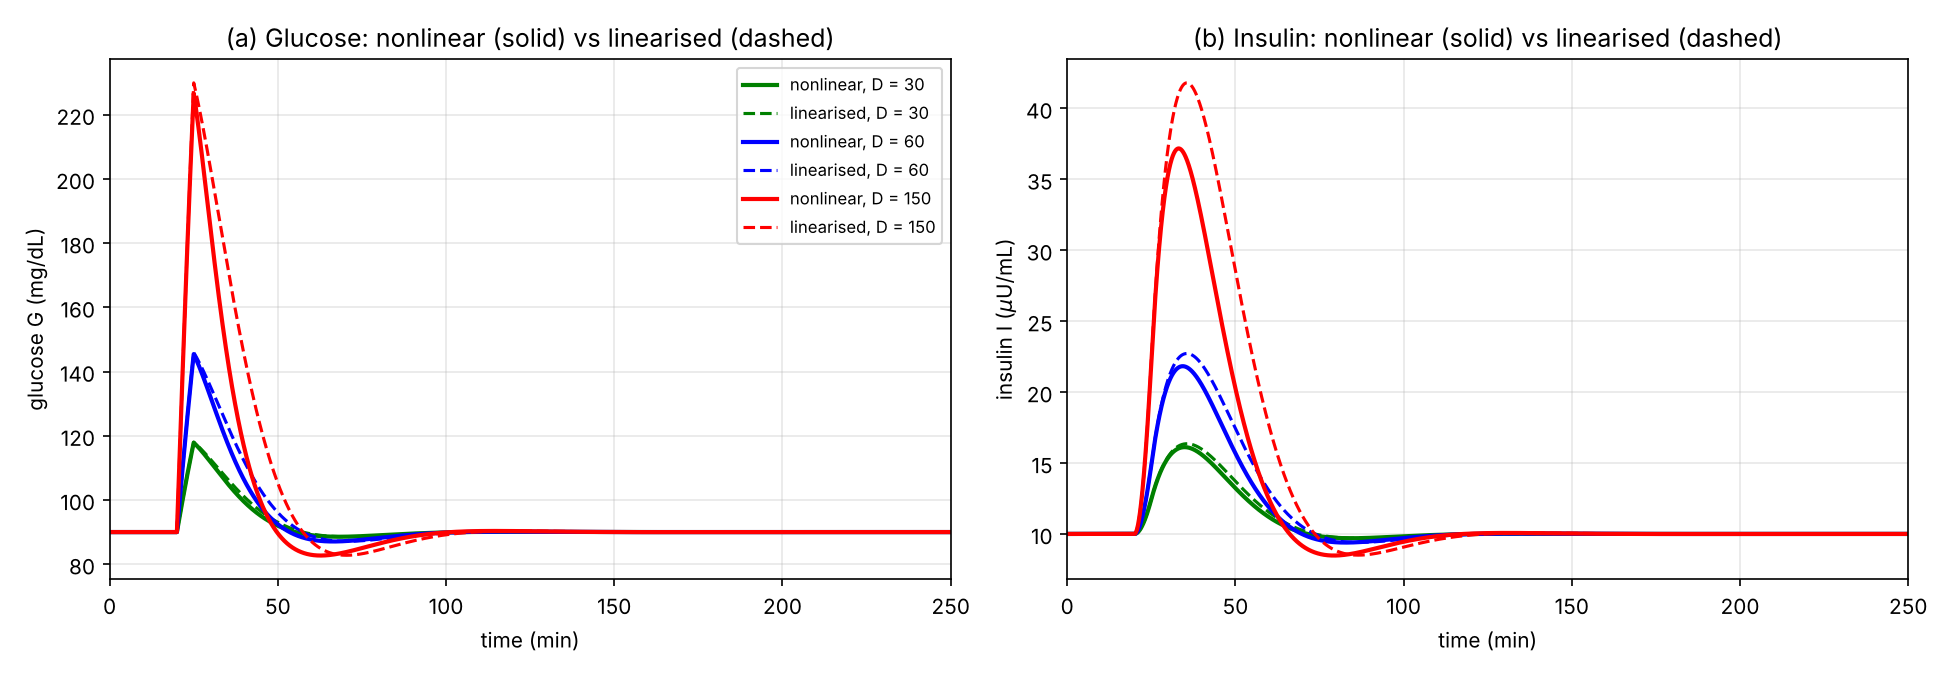
\includegraphics[width=\linewidth]{fig_nonlinear_vs_linear.png}
\caption{Nonlinear model (solid) and linearised model (dashed) for meals of $D=30$, $60$ and $150$\,mg/dL with $c=0.04$: (a) glucose, (b) insulin.}
\label{fig:nl_vs_lin}
\end{figure}

Since the eigenvalue analysis is based on the linear model, we wanted to see how close it is to the full model (Figure~\ref{fig:nl_vs_lin}). For a small meal ($D=30$) the largest difference in glucose is $1.6$\,mg/dL. For the normal meal ($D=60$) it is $5.9$\,mg/dL, and for a large meal ($D=150$) it is $29.7$\,mg/dL. The error grows roughly like $D^2$, which makes sense because the term we dropped, $-axy$, is quadratic. In the nonlinear model glucose falls faster after a big meal, since uptake depends on the actual glucose level rather than $\Gb$. But the overall shape (one peak, one small dip, return to normal) is the same, so the classification from the eigenvalues still holds for realistic meals.

%======================================================================
\section{What the Results Mean Biologically}\label{sec:bio_interp}

For a healthy person ($c=0.04$), our model gives a glucose peak of about $145$\,mg/dL after the meal, a return to normal within about an hour, a small dip of about $3$\,mg/dL roughly $45$ minutes after the meal, and an insulin peak about twice the fasting level. These are reasonable numbers. Real glucose tolerance test curves also often show a small dip below the fasting level, and Ackerman et al.\ \cite{ackerman} fitted this kind of damped oscillation to such test data.

When $c$ is below $\cs$, which is similar to early Type-2 diabetes or prediabetes where the $\beta$-cells respond weakly, glucose comes back slowly without any dip. The area under the glucose curve above $90$\,mg/dL goes from about $762$\,mg\,min/dL at $c=0.04$ to about $2234$ at $c=0.004$, almost three times more. So each meal exposes the body to much more glucose, and over years this is what damages tissues. Clinically this is called impaired glucose tolerance.

When $c$ is much larger than $\cs$, the response becomes weakly damped and glucose overshoots. We got minimum glucose values of $76$\,mg/dL for $c=0.15$ and $59$\,mg/dL for $c=0.4$, and the second one is below the $70$\,mg/dL hypoglycaemia limit. This is similar to reactive hypoglycaemia, where some people feel shaky, sweaty and hungry a few hours after eating because their insulin response is too strong. It is also seen after gastric bypass surgery, where glucose is absorbed very quickly.

So there is a trade-off. Too little insulin response means glucose stays high for too long, and too much means glucose dips too low. Our normal case ($\zeta\approx0.7$) sits in between, with one small dip and a fairly quick return. This matches the single small dip usually seen in a healthy person after a meal.

%======================================================================
\section{Extension: Type-1 Diabetes}\label{sec:type1}

\subsection{Model}
In Type-1 diabetes the pancreas does not make insulin, so we set
\begin{equation}
s_0=0,\qquad c=0 .
\end{equation}
The model becomes
\begin{equation}\label{eq:type1}
\frac{dG}{dt}=R_0-bG-aGI+M(t),\qquad \frac{dI}{dt}=-dI .
\end{equation}
The insulin equation now does not depend on $G$, and its solution is $I(t)=I(0)e^{-dt}$, so any insulin left in the blood is cleared within a few half-lives. With $I=0$ the glucose equation is $dG/dt=R_0-bG$, so the only equilibrium is
\begin{equation}
G^{*}=\frac{R_0}{b}=\Gb\Bigl(1+\frac{a\Ib}{b}\Bigr)=90\times4=360\ \text{mg/dL},\qquad I^*=0 .
\end{equation}
The healthy equilibrium $(90,10)$ does not exist any more.

\subsection{Stability}
At $(360,0)$ the Jacobian is
\begin{equation}
J=\begin{pmatrix}-b-aI^{*} & -aG^{*}\\ 0 & -d\end{pmatrix}
=\begin{pmatrix}-0.005 & -0.54\\ 0 & -0.1\end{pmatrix}.
\end{equation}
It is upper triangular, so the eigenvalues are just the diagonal entries, $\lambda_1=-0.005$ and $\lambda_2=-0.1$. Both are real and negative, so $(360,0)$ is a stable node. The system is still stable, but at the wrong glucose level. Without $c$ there is no $\beta c$ term in the determinant, so the eigenvalues are just the uncoupled rates. The glucose eigenvalue $-b=-0.005$ is very small, which means glucose drifts up to $360$ slowly, with a time constant of $200$ minutes. In terms of the model, this is what failure of homeostasis means: the feedback is gone, and glucose settles wherever the liver output and the insulin-independent uptake happen to balance.

\subsection{One meal}

\begin{figure}[H]
\centering
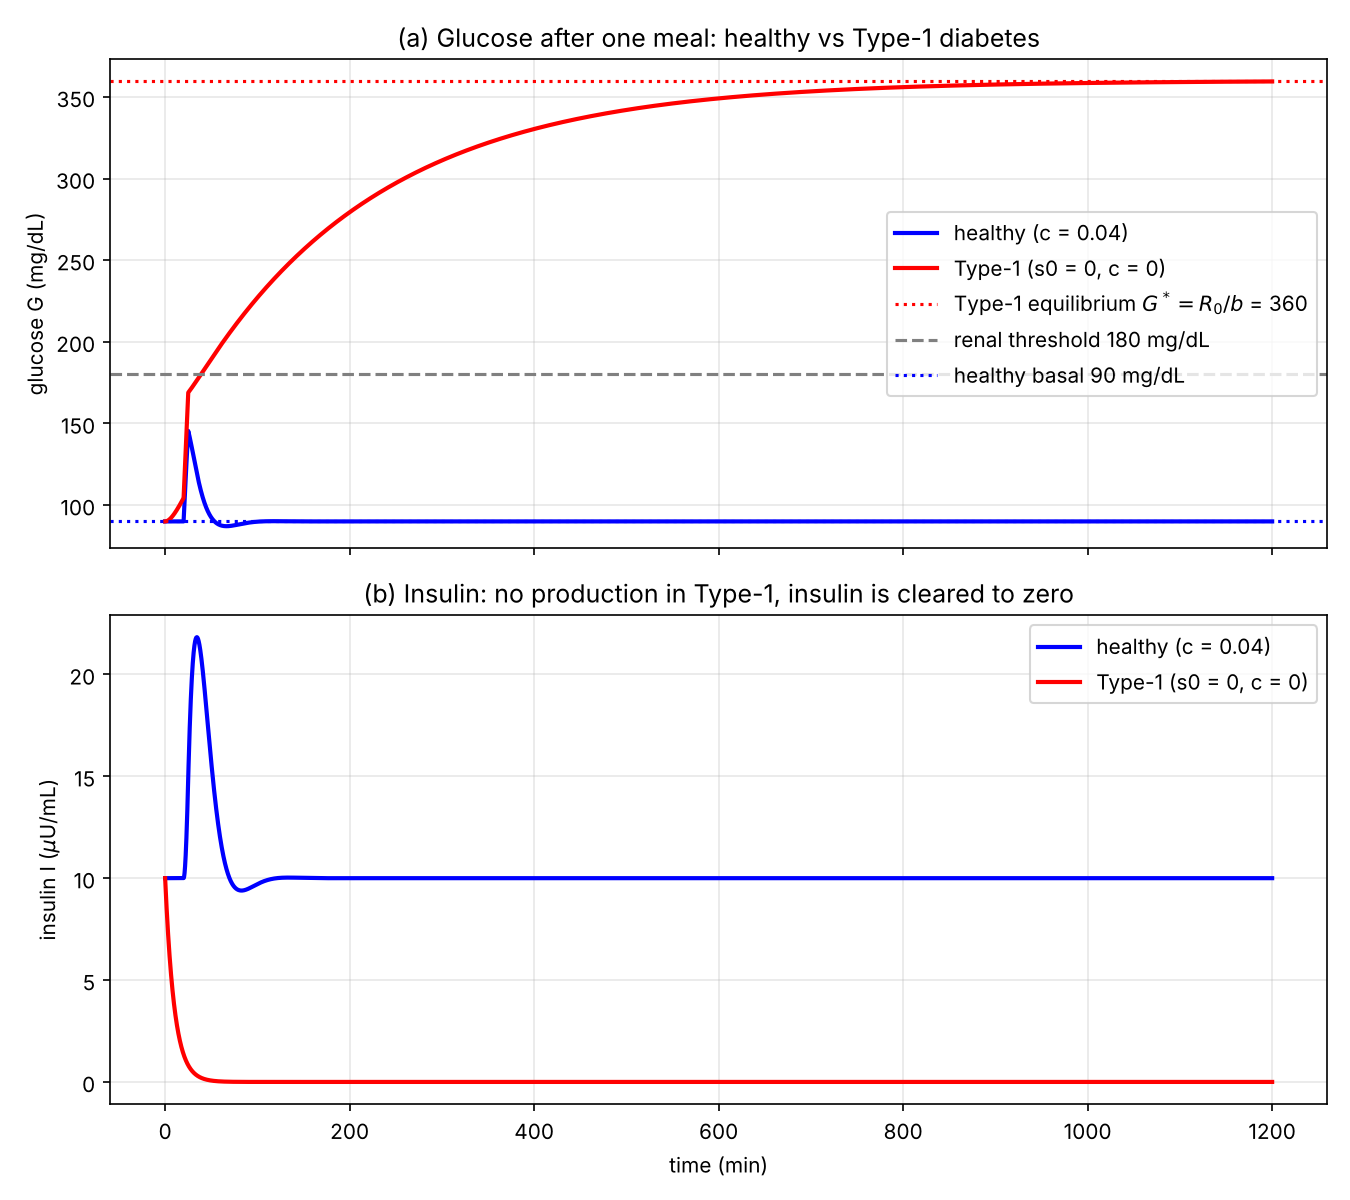
\includegraphics[width=0.82\linewidth]{fig_type1_single_meal.png}
\caption{One meal at $t=20$ for a healthy person and a Type-1 diabetic, both starting from $(90,10)$: (a) glucose, (b) insulin.}
\label{fig:t1_single}
\end{figure}

In Figure~\ref{fig:t1_single} the healthy case is the same as before. In the Type-1 case insulin drops to zero with a half-life of about $7$ minutes, and glucose starts going up even before the meal. The meal adds $60$\,mg/dL, but glucose does not come back down. It passes $180$\,mg/dL (the level where glucose starts appearing in urine) at $t=38.8$ minutes and keeps rising towards $360$. After $20$ hours it is at $359.5$\,mg/dL.

\subsection{Phase plane}

\begin{figure}[H]
\centering
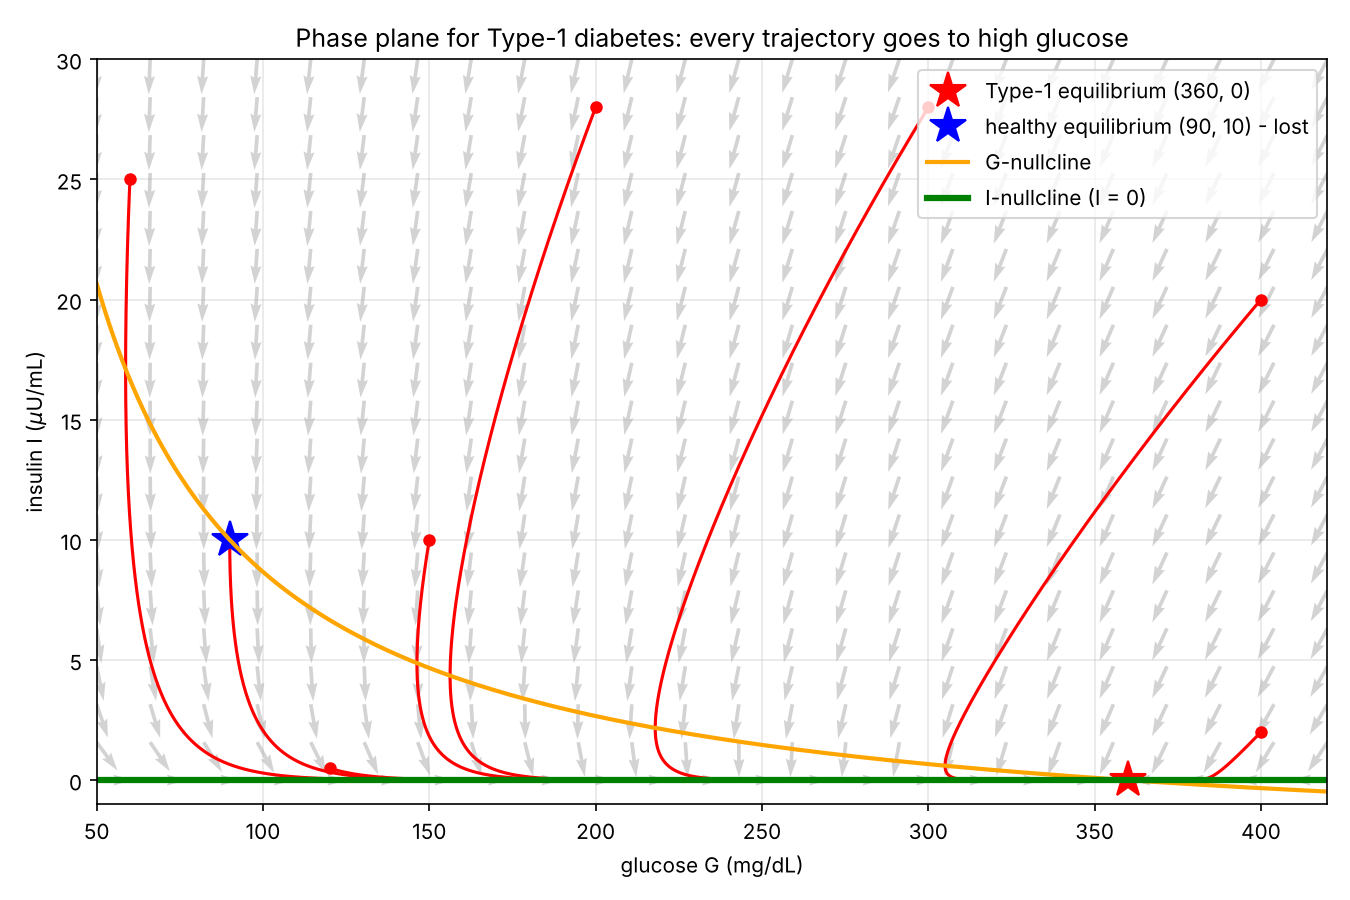
\includegraphics[width=0.78\linewidth]{fig_type1_phase.png}
\caption{Phase plane for untreated Type-1 diabetes. Red curves start from eight different points. The red star is the new equilibrium $(360,0)$ and the blue star is the old healthy point $(90,10)$, which is no longer an equilibrium.}
\label{fig:t1_phase}
\end{figure}

In Figure~\ref{fig:t1_phase} the $I$-nullcline is now just the line $I=0$, and it meets the $G$-nullcline only at $G=360$. Every trajectory, including the one starting from the old healthy state, first drops quickly towards $I=0$ (eigenvalue $-d$) and then moves slowly along the $G$-axis to $360$ (eigenvalue $-b$). Trajectories that start with a lot of insulin, like $(200,28)$, first move left because the leftover insulin lowers glucose for a while, but once it is cleared they turn around and go right. Compared with Figure~\ref{fig:phase_nl}, removing $c$ and $s_0$ completely changes the phase plane.

%======================================================================
\section{Division of Work}\label{sec:work}

\begin{table}[H]
\centering
\caption{Division of work.}
\label{tab:work}
\begin{tabular}{p{0.22\linewidth}p{0.2\linewidth}p{0.48\linewidth}}
\toprule
Member & Role & Contribution \\
\midrule
Akshith Hiremath & Endocrine Modeler & Biological background, assumptions, setting up equations \eqref{eq:G}--\eqref{eq:I}, choosing parameters, existence and uniqueness. \\
Snigdha Kanduri & Linearization Specialist & Jacobian, characteristic equation, exact solutions of the linear system, comparison of linear and nonlinear models. \\
Nairit Bansal & Eigenvalue Analyst & Discriminant and $\cs$, damping ratio, Table~\ref{tab:eig}, eigenvalue locus and plots against $c$. \\
Jayaditya Kushwah & Simulation Coder & RK4 solver, meal impulse and three-part solving, comparison with SciPy. \\
Aluri Venkata Sai Anirudh & Simulation Coder & Meal response and sensitivity simulations, Table~\ref{tab:metrics}, Type-1 simulations. \\
Khushal Kadyan & Trajectory Visualizer & Phase-plane plots, direction fields, nullclines and trajectories. \\
Shaan Sharma & Biological Interpreter & Biological meaning of the results, Type-1 diabetes extension. \\
\bottomrule
\end{tabular}
\end{table}

%======================================================================
\section{Limitations}\label{sec:limits}
Our model is quite simple, and there are several things it leaves out. Insulin in the body acts with a delay through the tissues, which more detailed models handle with a third variable; adding this or a time delay could also produce the slow natural oscillations seen in real glucose data, which a stable two-variable model cannot. We kept the liver's glucose output constant, while in reality insulin also reduces it. Real meals are absorbed over one to two hours, not five minutes, so a gut compartment would make the meal input more realistic. Our parameters are reasonable but not fitted to any patient data. Finally, to model Type-2 diabetes properly we would also need to reduce the insulin sensitivity $a$, not just $c$.

%======================================================================
\section{Conclusion}\label{sec:conclusion}
We modelled the glucose--insulin feedback loop with two coupled nonlinear ODEs and showed that the model has a unique fasting equilibrium and well-behaved solutions. Linearising gave the characteristic equation $\lambda^2+(\alpha+d)\lambda+(\alpha d+\beta c)=0$. From the trace and determinant the equilibrium is stable for any insulin production rate, and from the discriminant we found the critical value $\cs=(\alpha-d)^2/4\beta\approx0.0119$. Below $\cs$ the equilibrium is a node and glucose returns directly with no dip. Above it, it is a spiral and glucose oscillates on the way back. The eigenvalue locus and the simulations agree with this value.

Our RK4 code matched SciPy closely. The phase plots show straight-line approach along the eigenvectors in the node case and inward spirals in the spiral case.

Biologically, the healthy case is slightly underdamped ($\zeta\approx0.7$). Too little insulin response leaves glucose high for a long time, and too much causes dips that can reach hypoglycaemia. In Type-1 diabetes the feedback disappears, the healthy equilibrium is lost and glucose goes to $360$\,mg/dL.

%======================================================================
\section{Code and Figures}\label{sec:repo}
All our Python code, the figures and the program output are on GitHub:
\begin{center}
\url{\repourl}
\end{center}
The \texttt{code} folder has the five scripts from Section~\ref{sec:numerics} and \texttt{run\_all.py}, and the \texttt{figures} folder has every figure in this report along with the printed output (\texttt{run\_all\_output.txt}) used for Tables~\ref{tab:eig} and \ref{tab:metrics}. Running \texttt{python run\_all.py} inside the \texttt{code} folder regenerates everything.

%======================================================================
\begin{thebibliography}{9}
\bibitem{bolie} V.~W.~Bolie, ``Coefficients of normal blood glucose regulation,'' \emph{Journal of Applied Physiology}, 16(5):783--788, 1961.
\bibitem{ackerman} E.~Ackerman, L.~C.~Gatewood, J.~W.~Rosevear and G.~D.~Molnar, ``Model studies of blood-glucose regulation,'' \emph{Bulletin of Mathematical Biophysics}, 27:21--37, 1965.
\bibitem{boyce} W.~E.~Boyce and R.~C.~DiPrima, \emph{Elementary Differential Equations and Boundary Value Problems}, 10th ed., Wiley, 2012.
\end{thebibliography}

\end{document}
